\pagebreak
\section*{Executive Summary}
\addcontentsline{toc}{section}{Executive Summary}

Data Challenge 3 (DC3) is the third in a series of prototypes of the
LSST Data Management System (DMS). Through these data challenges, we
seek to identify the most challenging technical problems to building a
DMS that meets the LSST science goals. We prototype specific solutions
to these challenges with the expectation that by the start of the
construction phase of the telescope, we will have a well-defined plan
for how to build a DMS that can perform at the level needed by first
light. Despite the prototyping nature of the data challenges, we are
not producing throwaway code; rather, we expect that the software we
produce in the data challenges will serve as the foundation for the
DMS that will be completed during the construction phase.

\subsection*{DC3a in Context}

The DMS software architecture can be described as essentially
containing two types of components. One type is a component
representing a specific science application -- a discrete stage in the
series of steps needed to go from raw image data to science
result. The other type of component is part of the infrastructure
which orchestrates the execution of the science app stages, provides
the necessary data I/O, allows logging capabilities, and allows for
the parallel distribution of the science computation. We refer to the
first class of components as the \textit{science applications} and the
second class as the \textit{middleware} or \textit{infrastructure}; a
collected series of sequential steps is called a \textit{pipeline}.

In Data Challenge 1 (DC1), we focussed on the DMS middleware design
for supporting nightly processing; this software scaffolding ---
the \textit{pipeline framework} --- modeled the infrastructure
necessary to support science algorithms but did not actually execute
them, using instead \textit{resource consumers}, which simulated the
expected computational node of the algorithms but produced no useable
science output.  In Data Challenge 2 (DC2), we replaced the resource
consumers with real implementations for the most challenge aspects of
image processing and alert production. We also updated the pipeline
harness framework as development of the scientific algorithms revealed
new framework requirements.

The scope of DC3 is significantly larger than that of the previous
data challenges, including both a more capable implementation of the
Alert Production and a first prototype implementation of the Data
Release Production.  Because of the large scope of DC3, we have
divided it into two phases, DC3a and b.  DC3a includes only the Alert
Production capabilities, while DC3b adds the Data Release Production.
Other goals of DC3a include improvements to the application framework
and middleware, along with the following new capabilities: the
Instrument Signature Removal (ISR) pipeline, World Coordinate System
(WCS) determination within the Image Characterization (IC) pipeline,
and an initial SDQA system. Also improvements were sought in both the
science quality and the execution speed of the science applications,
as well as new capabilities within the software build system.

\subsection*{Results}

DC3a Alert Production was composed of three loosely coupled pipelines
that communicated with each other through asynchronous messages ({\it
events}) and a common database.  The three pipelines were:
\begin{itemize}
\item IPSD, handling image processing and source characterization
\item NightMOPS, which predicted positions of moving objects
\item Association (ap), which associated detected sources with known objects
\end{itemize}

\begin{table}[bp]
\centering
\caption{Summary of Production Runs analyzed in this report
\label{tbl:runsummary}}
\vspace{\baselineskip}
\begin{tabular}{rccccc}
\hline\hline
          &         &       & \multicolumn{3}{c}{Images Processed: Num/Size} \\
runId     & nVisits & nAmps & Raw Images & Ancil. Images & Output Images \\ \hline
rlp1233   & 85      & 31  & 5146/24 GB    & 88/13 GB       & 60525/240 GB \\ 
rlp1234   & 85      & 31  & 5146/24 GB    & 88/13 GB       & 60525/240 GB \\ 
rlpabe041 & 12      & 288 & 3456/33 GB    & 15/2 GB        & 79368/313 GB \\ \hline
Total     & ---     & 250 & 13748/81 GB   & 191/28 GB      & 2000418/793 GB \\ \hline
\end{tabular}
\end{table}

We executed many short runs of the pipelines for purposes of
performance analysis, quality analysis, and debugging, resulting in
important algorithm optimizations as well as numerous bug fixes. As in
DC2, the astronomical images we used as input were from the CFHT-LS
Deep Survey fields D3 and D4.  We also executed some but not all
stages using images from the simulated data collections, SimWide and
SimDeep, and these runs were instrumental in understanding and
correcting processing problems.

We then executed larger-scale DC3a production runs on clusters at
NCSA.  For final analysis of data quality and processing performance,
we have concentrated on two production runs on the NCSA LSST
development cluster (referred to by their run
identifiers, \texttt{rlp1233} and \texttt{rlp1234}. These runs used
identical versions of the software and configured identically, but
processing a different set of 31 amplifiers in the focal plane for 85
visits to the CFHT-LS D3 field.  To collect explore the scalability of
the pipelines, we also executed runs of the image processing pipeline
on the NCSA cluster Abe.  These runs were performed across 36 8-core
nodes, processing the entire 288-amplifier focal plane for CFHT-LS
simultaneously.  (Some of the supporting software services, such as
the event broker and the database, remained on the NCSA LSST cluster.)
These runs showed that the pipelines scaled reasonably well to this
level, although running at this scale did reveal some additional
configuration requirements for the events broker and the MySQL
database.  To run on Abe, we needed integrate grid-based technologies
(including grid-based job management using Condor-G) into our the
pipeline orchestration layer.

The Abe runs also allowed us to demonstrate successful use of the 
Lustre parallel filesystem.  As in DC2, Lustre proved unstable  on the
LSST development cluster under heavy I/O, and schedule and hardware
resource limitations prevented us from exploring the causes in 
any detail.  As a result that the LSST development cluster runs were
all performed under the NFS shared file system.  However, Lustre
worked well on the Abe cluster. 

\subsubsection*{Science Data Quality}
We evaluated the science data quality of DC3a in three areas that are
judged to be the most demanding for the software system to meet, 
and are each directly related to science requirements. 
\begin{itemize}
\item WCS accuracy
\item Difference image quality
\item Difference image lightcurve quality
\end{itemize}
\paragraph{WCS Accuracy}
The World Coordinate system (WCS) is a geometrical mapping between
image pixel coordinates and sky coordinates.  An accurate WCS is the
foundation for processing steps such as image coaddition, image
differencing, and the fitting of astrometric models. Within the
context of DC3a, the WCS has an especially direct effect on the
quality of the difference images.  

The WCS quality was evaluated in an automated way with a program that
checked every image that was processed.  The WCS-predicted sky
coordinates of stars in the images were compared with the catalog
positions of the same stars.  The level of the discrepancies measure
the WCS quality. The results of the analysis for the two benchmark
DC3a runs show that 

\begin{itemize}
\item Most images result in acceptable WCS quality, with median errors
  of about 40 milli-arcsec
\item A small number of images have a failed WCS, which is in error by
  many arcsec.
\end{itemize}
For the two benchmark runs, there were respectively 109 failures out
of 2629 images processed (4\%), and 14 out of 2509 (0.5\%).  The
causes of the failures will be investigated during the DC3b planning
process.  Additionally, we will set more stringent WCS quality goals
for DC3b, since they will be required for full data release processing.


\paragraph{Difference Image Quality}

To investigate difference image quality, a representative subset of
the DC3a difference images were first visually inspected.  They fall
into three distinct categories. First, difference images produced from
images with failed WCS's show either ``bipolar'' subtractions in the
case of marginal failures or completely nonfunctional subtractions in
the case of extreme WCS failures.  Images with successful WCS's
generate subtractions that look good except in the vicinity of bright
stars,where a high spatial frequency pattern is evident.

We leave aside the roughly 2\% of
the difference images that involved WCS failures, since they tell us
little about the performance of the difference image algorithm itself.
In the absence of variable or moving sources, an ideal difference
image will have a mean of zero, and show uncorrelated random
fluctuations at the level expected from the variance of the input
images.  We therefore defined a ``figure-of-merit image'' as the ratio
of the difference image to the expected fluctuation level, which
varies with the flux in the input image.
A plot along a horizontal line through
the subtracted bright star in a typical figure-of-merit image is shown in
Figure 1.  This plot shows several aspects of the difference
image quality:

\begin{itemize}
\item The average level of the image is near zero, as expected
\item Away from bright stars, the level of the noise is near 1.0, the
  expected value
\item In the footprint of bright stars, the noise is larger than
  expected by a large factor, about 20 in this particular case.
\end{itemize}  

The large residuals in the footprint of bright stars cause problems
for downstream alert processing, and are believed to result from the
kernel basis functions chosen for the image subtraction algorithm.
For DC3b, we will ensure that these residuals are greatly reduced.

\begin{figure}[hb]
\begin{center}
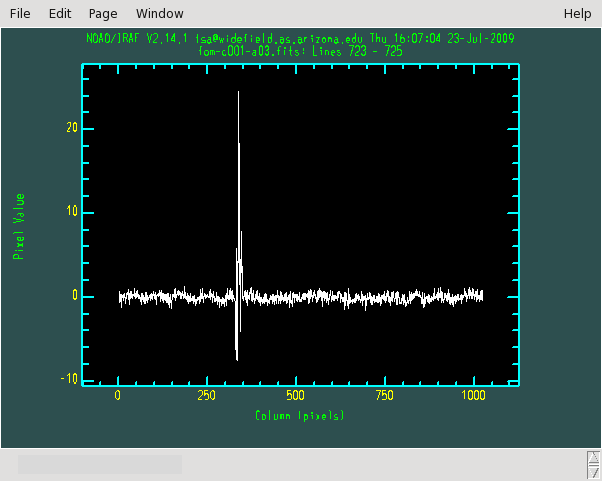
\includegraphics{images/rlp1233_v695833-e0-c001-a03-fom_plot.png}
\caption{Line section through figure-of-merit image for
  rlp1233/695833-e0-c001-a03.  The line is chosen to pass through a
  subtracted bright star at (338,725)}
\label{Figure 1}
\end{center}
\end{figure}

\paragraph{Difference Light Curve Quality}
Leaving out images that had WCS failures, run rlp1233 yielded 63000
objects with difference sources detected above threshold in at least
one visit. The number of visits
for which difference sources were detected varies widely with the object, between 1 and
about 75.  The latter number is close to the number of visits
processed in rlp1233, which is 85.  Spot checking of these sources in
the images suggests that the vast majority are the result of artifacts
in the difference images, with residuals around bright stars being the
most frequent cause.  The highly structured nature of the difference
image residuals, combined with the relatively large kernel footprint,
causes further artifacts, since multiple peaks can be detected in a
single footprint.  In general, though it will certainly be the case
that real astrophysical signals from variable stars and transient
events are present in this data, it is currently impractical to
separate them from the noise with the analysis tools readily
available.  We expect that improvement of the difference image
algorithm for DC3b will fundamentally improve this situation, allowing
science quality to be meaningfully assessed against requirements.

\subsubsection{Processing Performance}

As in DC2, we use the logging framework (in which every log message is
time-stamped) to instrument our pipeline processing code.  We can
calculate how much time is spent on the different contributors to the
overall processing time, including I/O, middleware overhead,
scientific processing.  Table \ref{ex:tbl:visitstats} summarizes the
average time to process a visit through each pipeline: the left set of
values represents the total time per visit (neglecting time waiting
for new data to process), the right set looks strictly at time spent
in application-level code.  As one can see, the overhead added by the
pipeline framework is minimal.  While the total processing time per
visit is longer than in DC2, we note that DC3a does more processing,
including additional caching of intermediate results that would not be
necessary in production mode.  When we examine the common stages of
processing in DC2 and DC3a, we see large improvements across the
board, along with a much lower variation in processing times over
different data.  The most expensive stage, image subtraction, saw a
2-fold improvement over DC2; subsequent experiments showed tuning
configuration parameters increases that factor to 3.

\begin{table}[ht]
\begin{center}
\caption{Average Processing Times Per Visit
\label{ex:tbl:visitstats}}
\vspace{\baselineskip}
\begin{tabular}{ l | c | c |}
\hline\hline
          & Total Processing Time, corrected
          & Application Processing Time \\ 
Pipeline  & average $\pm$  $3\sigma$ (s) & average $\pm$ $3\sigma$ (s) \\ \hline
IPSD      & 264.7 $\pm$ 20.2 & 264.1 $\pm$ 20.1  \\ 
nightmops & 10.6  $\pm$  4.4 & 10.4 $\pm$  4.4  \\ 
ap        & 1.4   $\pm$  0.7 & 1.2 $\pm$  0.7  \\ \hline
\hline
\end{tabular}

\end{center}
\end{table}

Comparing the small runs on the LSST development cluster to the larger
one on the Abe cluster shows overall good scaling.  When we
concentrate on the stages that are dedicated to applying science
algorithms, we see that most of them (including image subtraction)
appear to scale near-perfectly, as shown in
Table \ref{ex:tbl:allscislices}; though, three stages show some
degredation.  

\begin{table}[htbp]
\begin{center}
\caption{IPSD: Average Processing Times (s) Per Stage. 
\label{ex:tbl:allscislices}}
\vspace{\baselineskip}
\begin{tabular}{llcrrc|crr|c}
\hline\hline
   &      && \multicolumn{2}{c}{{\tt rlp1233} \& {\tt rlp1234}} 
         &&& \multicolumn{2}{c|}{{\tt rlpabe041}} & \\
\# & Name && \multicolumn{1}{c}{average}&\multicolumn{1}{c}{$3\sigma$} 
         &&& \multicolumn{1}{c}{average}&\multicolumn{1}{c|}{$3\sigma$} 
   & Speed-up$^a$ \\ 
\hline
12 &                 isr0 &&  1.514 &  0.113 &&&  1.389 &  0.275 & 1.1 \\  % -
13 &      sourceDetection &&  1.638 &  0.110 &&&  1.479 &  0.465 & 1.1 \\  % - 
15 &    sourceMeasurement &&  0.232 &  0.772 &&&  0.234 &  1.184 & 1.0 \\  % 0 
17 &     psfDetermination &&  0.112 &  0.120 &&&  0.107 &  0.123 & 0.9 \\  % 0 
25 &                 isr1 &&  1.585 &  0.163 &&&  1.439 &  0.184 & 1.1 \\  % 0 
27 &     wcsDetermination &&  0.172 &  0.085 &&&  0.191 &  0.403 & 0.9 \\  % 0 
35 &     imageDifference0 && 71.174 & 15.573 &&& 62.082 & 14.898 & 1.1 \\  % - 
36 &     imageDifference1 && 69.289 & 15.198 &&& 61.069 & 15.717 & 1.1 \\  % - 
38 &         addAndDetect &&  7.851 &  0.680 &&&  9.354 &  3.400 & 0.6 \\  % + 
39 & diaSourceMeasurement &&  0.114 &  0.610 &&&  0.261 &  2.979 & 0.4 \\  % + 
41 & sourceClassification &&  0.005 &  0.005 &&&  0.008 &  0.029 & 0.8 \\  % + 
\hline
\multicolumn{10}{l}{$^a$where 1 represents perfect scaling; values $> 1$ reflect the slightly better hardware in}  \\ 
\multicolumn{10}{l}{\phantom{$^a$}the Abe cluster}  \\ 
\end{tabular}
\end{center}
\end{table}

The comparison of the runs also reveals interesting results for stages
handling I/O, particularly when we consider filesystem and database
I/O separately.  Due to the problems we encountered using the Lustre
parallel filesystem on the development cluster, the smaller runs were
done using NFS.  This filesystem is known to perform poorly under most
conditions, and our results bear this out.  On the other hand, the
file-based I/O performance of the Lustre filesystem on Abe performed
very well, reading 9 times more data in the same or less time.  The one
exception was the stage in which all parallel processes had to read
the same template image at the same time; here, redundanly reading 9
times the data took twice as long.  More scaling experiments are
planned to understand file-based I/O performance.  

Database performance dropped as we went to the large run on Abe.  It
appears that this is in large part due to network latency effect since
the database ran on the development cluster while the pipeline ran on
Abe.  This bears more experiments because we cannot yet tell what the
contribution to the time comes from having nine time the number of
simultaneous database clients.  No special parallelizing of database
access was in place.  

Overall, we will need to spend more effort developing good I/O
strategies in future data challenges.  In particular, we need
experiment more with optimizing the use of parallel filesystems and
deploying distributed databases.  


